% -*- coding: cp932-dos -*-
\documentclass{jarticle}

\usepackage{icspresen_m22}
\usepackage{comment}
\usepackage{longtable}
\usepackage{latexsym}
\usepackage[dvipdfmx]{graphicx}
\usepackage{url}
\usepackage{caption}

\No{}
\Jtitle{英単語タイピングゲームによるスペリング誤りの抽出と分析}
\Etitle{Extraction and analysis of spelling errors using English word typing game}
\Author{12890526___立花_竜一_______________指導教官__小町_守_准教授}
\presenyear{27}
\presendate{平成27年9月2日}
\master   % 修士論文発表会の場合
%\bachelor % 特別研究発表会の場合

\captionsetup[figure]{format=plain, labelformat=simple, labelsep=period, font=small}
\captionsetup[table]{format=plain, labelformat=simple, labelsep=period, font=small}

\begin{document}
\mktitle
%
\renewcommand{\baselinestretch}{1.1}\small
%

\section{はじめに}
\fontsize{9.37pt}{1pt}\selectfont
パソコンは主にキーボードを利用して操作を行うが,キーボードを利用する場合,スペリングを誤ってしまうことがある.たとえば,隣接するキーを誤って押してしまう混同や,アルファベット同士の音韻的・視覚的類似性によって間違えてしまう誤りがある.本研究ではキーボードの誤操作によって発生するタイポと誤認識によって発生する綴りの混同を合わせて\textbf{スペリング誤り}と定義する.

パソコンの普及率の向上に伴い,スペリング誤りの検出・訂正が注目され,スペリング誤りを分析してその原因を解明しようとする研究やスペリング誤り訂正に寄与する研究が行われている.たとえば,Twitterなどのwebサービスからスペリング誤りの候補を抽出する\cite{aramakiNLP2010},クラウドソーシングを利用した入力ログからスペリング誤りの候補を得る\cite{babaACL2012}などしてスペリング誤りの獲得を行う研究がある.
しかしコーパスから教師なしにスペリング誤りの候補を抽出する場合何の単語のスペリング誤りかわからない,クラウドソーシングを利用する場合コストがかかるといった難点があった.

一方ゲームにおいて用いられている要素をタスクに活用することによって,ユーザがタスクにより取り組んでもらえるようにタスクの設定を工夫するゲーミフィケーションの研究が盛んになってきている\cite{deterdingACM2011}.教師なしに知識獲得をするのと異なり,ゲーミフィケーションでは自分でタスクを設定することができる利点がある.また,ゲーミフィケーションではユーザに対価を払うことなく,何らかのタスクにおいてのリソースを獲得できるという利点がある.

そこで本研究ではタイピングゲームを利用することで,スペリング誤りに対応した単語は何か分かっており,コストもかからないスペリング誤りの抽出手法を提案し,抽出したスペリング誤りに関する分析を行う.

本研究の主要な貢献は以下である.

\begin{itemize}
 \item 我々の知る限り,タイピングゲームをスペリング誤り抽出に用いた研究は本研究が初めてである.
 \item ユーザが入力しようとしている英単語がわかっているため,編集距離に基づくスペリング誤り抽出手法\cite{aramakiNLP2010}では行えないようなスペリング誤りに関しての分析が行える.
\end{itemize}

 \begin{table*}[t]
  \small
  \centering
   \caption{ユーザが入力した文字列と文字列に対応した英単語の比較とスペリング誤りの抽出例}
   \begin{tabular}{|c|c|c|c|c|c|} \hline
       	ユーザが入力した文字列 & 文字列に対応した英単語 & スペリング誤り & 1つ前の文字 & 入力すべき文字 & 1つ後の文字\\ \hline
	    bel\underline{e}ief & belief & e & l & i & e\\ \hline
   \end{tabular}
 \end{table*}

\section{関連研究}
まずスペリング誤りに関しての関連研究について説明する.
KernighanらはNoisy Channel Modelを使って単語が与えられたときの訂正候補の確率をモデル化することでスペリング訂正を行った\cite{kernighan1990spelling}.この研究ではスペリング訂正モデルは1文字同士の挿入,削除,置換,転置といった編集距離の値に基づいて計算された.またBrillらはKernighanらと同様にNoisy Channel Modelによるスペリング誤りの訂正を行ったが,訂正候補の確率をモデル化するときに一文字だけでなく,文字列の編集距離を考慮することでスペリング誤りの訂正の精度を向上させた\cite{brill2000improved}.
Ahmadらはウェブ検索クエリログからスペリングを訂正するためのモデルを自動的に学習した\cite{ahmad2005learning}.この研究ではEMアルゴリズムを手法とすることで,正解データを必要とせずに重み付き編集距離を学習した.
重み付き編集距離はaとeは誤りやすいが,aとlは誤りにくいといった文字同士の誤りやすさに関する情報を反映するために利用される.
\begin{comment}
Ahmadらはまず重み付けされていないモデルを用いて誤りを検出し,その誤りを用いてモデルの重み付けを更新することで学習を行った.
\end{comment}
これらの研究ではスペリング誤りの訂正のために研究を行っているが,本研究ではスペリング誤りの訂正は行わず,スペリング誤りの特徴の分析を行っている.

Cookによる研究\cite{cook1997l2}では英語を母語とする第一言語話者と母語としない第二言語話者の英語のスペリング誤りを比較して分析を行っている.本研究では英語を母語としないユーザのスペリング誤りを分析している点が共通しているが,Cookはスペリング誤りのデータを学生がテストや宿題で書いたものなどから抽出していたのに対し,本研究ではタイピングゲームを用いてスペリング誤りを抽出する.

 \begin{table*}[t]
  \small
  \centering
   \caption{スペリング誤りと判定される文字列,されない文字列と複数のスペリング誤りが抽出される文字列の例}
   \begin{tabular}{|c|c|c|c|} \hline
       	ユーザが入力した文字列 & 文字列に対応した英単語 & スペリング誤りの文字 & スペリング誤りの文字列\\ \hline
		in\underline{g}cre\underline{s}ase & increase & gとs & \\ \hline
		\underline{inly}only & only & i & \\ \hline
	    bi\underline{yy}t & bit & yとy & yy\\ \hline
   \end{tabular}
 \end{table*}

荒牧らはTwitterのクロールデータを利用することで英単語のスペリング誤りの抽出を行い,スペリング誤りの原因を分析した\cite{aramakiNLP2010}.またスペリング誤りとスペリング誤りでないものを判別する学習器を構築し,実験を行うことで分析結果の検証を行った.クロールしたデータにおいてスペリング誤り候補を決定するために,英単語から編集距離が1であるものを収集した.
本研究における荒牧らの研究との共通点は,キー配置によるスペリング誤りや単語内のスペリング誤りの位置といった観点でスペリング誤りの分析を行うことである.また荒牧らの研究では正解の単語を推測するために編集距離を利用していたが,本研究では正解の単語を推測する必要がない手法を提案する.

Babaらはクラウドソーシングの1つであるAmazon Mechanical Turkを利用して,ある画像が何を描写しているかユーザに英文を入力させユーザのキーストロークを抽出し,スペリング誤りに対応する単語が分かるスペリング誤り候補を抽出する手法を実装し,その結果に対して分析を行った\cite{babaACL2012}.修正前文字列と修正後文字列の編集距離が2以下であるものを抽出し,それらを比較してスペリング誤り候補を抽出することで分析を行った.本研究とはスペリング誤りに対応する単語がわかっている点が同じだが,この研究ではAmazon Mechanical Turkを利用するためコストがかかるのに対し,本研究ではコストのかからないタイピングゲームを用いたスペリング誤りの抽出手法を提案する.

またユーザがゲームを行うことを通して言語資源を得るという研究がある.Kumaranらはある句に対して同じ意味の句を得るためにユーザにゲームを行わさせた\cite{kumaranCOLING2014}.そのゲームはあるユーザがある句に関しての絵を描き,その絵を他のユーザに見せてその絵が何の句を示しているのか答えてもらうというものであった.
Vannellaらは意味的な知識の検証と拡張のために2つのゲームを作成し,ユーザに行わさせた\cite{vannella2014validating}.2つのゲームはそれぞれシューティングゲームとロールプレイングゲームを模したものであり,それらのゲームを行うことで概念同士の,または概念と画像の関係のアノテーションを行わせた.ユーザがゲームを通して行ったアノテーションは,クラウドソーシングにおいて労働者が報酬を受け取って作成したアノテーションと比較しても高い品質のものであった.
VenhuizenらはWordrobeと呼ばれるゲームをユーザに行わせることで語義のラベル付けを行った\cite{venhuizen2013gamification}.ゲームは語義に関する複数の選択がある質問の集合で構成されていて,複数のユーザはそれに答えて,他のユーザと答えが一致しているかどうかによってユーザが獲得する得点が決まる.
\begin{comment}
得られたデータの量は比較的少なかったが,適合率と再現率の結果は期待できるものであるとしている.
\end{comment}
これらの研究と本研究との共通点はゲームを用いて言語知識獲得を行う点であるが,相違点は得ることができる言語資源がスペリング誤りである点である.

\section{タイピングゲームによるスペリング誤り抽出}
本研究ではユーザがタイピングゲーム\footnote{\url{http://cl.sd.tmu.ac.jp/~ryu/typing_game.html}}を行うことで,ユーザがタイプしたアルファベットの文字列を抽出し,その文字列に対応した英単語と比較を行うことでスペリング誤りの獲得を行う.ユーザが入力する文字列にはスペリング誤りが含まれているため,ユーザがタイプしたアルファベットの文字列と英単語を比較することでスペリング誤りの分析が可能になる.

ユーザが入力したアルファベットの文字列とその文字列に対応した英単語の比較は,タイピングゲームにおいて間違いだと判定される文字を抽出するように比較が行われる.例えば表3.1ではユーザが入力した文字列とその文字列に対応した英単語の比較例を示している.入力すべき英単語はbeliefだったが,ユーザが実際に入力した文字列はbel\underline{e}iefであったとき,beliefの4文字目にあたるiを入力すべきときにアルファベットeを入力しているので,アルファベットeをスペリング誤りとして抽出を行う.スペリング誤りのアルファベットeと,ユーザが入力しようとしていたbeliefの4文字目にあたるiと,その前後の文字をスペリング誤りの原因の分析のためにそれぞれ抽出する.

ユーザが入力した文字列において複数のスペリング誤りが存在し,それらがタイピングゲームにおいて正解だと判定される文字または文字列で区切られている場合はそれぞれのスペリング誤りは別々のスペリング誤りとして扱うものとする.表3.2では1つの文字列において複数のスペリング誤りが抽出される例を示しており,ユーザが入力した文字列in\underline{g}cre\underline{s}aseにおいて3文字目のgと7文字目のsをスペリング誤りとして抽出している.3文字目のgをスペリング誤りとして扱ったあと,ingcresaseにおいて4文字目から6文字目creは文字列に対応した英単語increaseの3文字目から5文字目と対応して,タイピングゲームにおいて正解だと判定される.そのあとユーザは英単語increaseの6文字目の文字aを入力する必要があるが,ユーザは文字列ingcresaseの7文字目のsを入力しているので,結果gとsがスペリング誤りとして抽出される.

タイピングゲームにおいてユーザがスペリング誤りだと判定される文字を連続で入力する場合もあるが,その場合連続した文字列がタイピングゲームにおいて入力すべき文字以降の英単語の部分文字列であれば,その文字列はスペリング誤りとは判定せずに分析を行う.表3.2にはスペリング誤りと判定されない場合の文字や文字列の例が示されており,ユーザが入力した文字列は\underline{inly}onlyで,文字列に対応した英単語はonlyなので,タイピングゲームにおいて間違いだと判定される文字はそれぞれiとnとlとyであるが,inlyにおいて文字列nlyはそれぞれ入力すべき文字o以降の部分文字列なので,文字列nlyはそれぞれスペリング誤りとして抽出をしないものとする.

また表2にはスペリング誤りと判定される文字列の例が示されており,ユーザが入力した文字列bi\underline{yy}tから抽出されるスペリング誤りの文字としてyが2文字抽出され,入力すべき文字はtとする.

\begin{figure}[t]
	\centering
		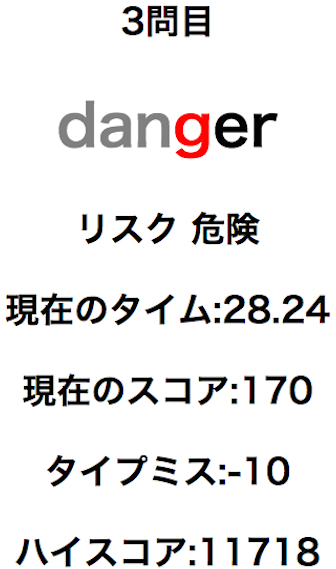
\includegraphics[width=3cm]{game2.png}
		\caption{タイピングゲームのスクリーンショット}
		\label{LabelExa}
\end{figure}

 \begin{table*}[t]
  \small
  \centering
   \caption{スペリング誤りの文字と頻度(入力すべき文字が語頭または語末の場合は\_を示す)}
   \begin{tabular}{|c|c|c|c|c|c|c|c|} \hline
       	スペリング誤りの文字 & 頻度 & 1つ前の文字 & 頻度 & 入力すべき文字 & 頻度 & 1つ後の文字 & 頻度\\ \hline
	    e & 93 & r & 14 & r & 17 & e & 36 \\ \hline
	    r & 73 & e & 12 & e & 19 & r & 26 \\ \hline
	    s & 67 & \_ & 21 & c & 17 & e & 15\\ \hline
	    i & 60 & \_ & 9 & o & 18 & i & 30\\ \hline
	    o & 59 & \_ & 19 & p & 12 & o & 24\\ \hline
	    n & 56 & i & 24 & o & 22 & n & 40\\ \hline
	    a & 54 & \_ & 14 & e & 10 & a & 22\\ \hline
	    t & 54 & g & 9 & h, r & 8 & t & 21\\ \hline
	    u & 35 & o & 8 & y & 11 & u & 14\\ \hline
	    d & 34 & \_ & 7 & s & 10 & \_ & 8\\ \hline
	    g & 34 & n & 11 & t & 8 & \_ & 17\\ \hline
	    l & 31 & m & 6 & p & 9 & l & 21\\ \hline
	    h & 25 & \_ & 7 & f & 5 & h, o & 5\\ \hline
	    v & 25 & \_ & 9 & b & 12 & e & 11\\ \hline
	    p & 24 & l, t & 5 & o & 16 & p & 5\\ \hline
	    y & 23 & a & 4 & t & 9 & y & 9\\ \hline
	    c & 20 & e, i & 4 & v & 6 & c, e & 6\\ \hline
	    k & 20 & a & 8 & l & 14 & \_ & 9\\ \hline
	    w & 20 & \_ & 8 & e & 14 & w & 5\\ \hline
	    b & 15 & i & 4 & v & 9 & e & 9\\ \hline
	    m & 14 & \_ & 4 & n & 4 & m & 3\\ \hline
	    f & 11 & \_ & 5 & r & 3 & \_ & 3\\ \hline
	    x & 3 & e, n, o & 1 & c & 2 & e & 2\\ \hline
	    j & 3 & c & 2 & k & 2 & \_ & 2\\ \hline
	    z & 2 & e, \_ & 1 & a, v & 1 & i, m & 1\\ \hline
	    q & 1 & p & 1 & e & 1 & c & 1\\ \hline
   \end{tabular}
 \end{table*}

\section{タイピングゲームの設計と実装}

この節ではタイピングゲームの設計と実装に関して説明する.

\subsection{タイピングゲームの設計}
タイピングゲームは図1のように表示され,ユーザは表示されている英単語を入力していく.ユーザが任意のキーを入力したときにゲームが開始され,それと同時にタイピングゲームにかかる時間の計測が始まる.英単語は既に入力し終わっている文字を灰色,スペリングを誤った文字を赤色,まだ入力していない文字を黒で示している.1つの英単語を入力し終わるごとに新たな単語が表示される.100単語タイプし終わるとゲームクリアとなる.スコアはスペリングを誤るたびに10点減点され,100問タイプし終わった時間が速いほど加点される.プレイに応じてユーザの現在のタイムやスコアも表示される.ユーザがタイピングゲームを行った中で最も高いスコアはハイスコアとして表示される.またスペリングを誤ったときや英単語を1単語入力し終わる度に効果音が鳴る.

\subsection{タイピングゲームの実装}
「初めて学ぶ人のためのJavaScript入門:タイピングゲームを作る」\footnote{\url{http://www.pori2.net/js/key/3.html}}を参考にしてタイピングゲームの実装を行った.サイトではユーザのキーコードの入力を受けてその入力が表示されているアルファベットと一致しているかどうかを判定し,ユーザがアルファベットを200文字正しく入力するまでの時間を計るアルゴリズムを示すソースコードが書かれている.本研究ではそのコードを以下のように改変・追加することで,研究のためのタイピングゲームの実装を行った.

まずユーザに入力させていたアルファベットを英単語に変更した.
次にユーザが正しく英単語を入力したときは正解を示す効果音,スペリング誤りをしたときは不正解を示す効果音が鳴る機能を実装した.またユーザが英単語をタイプしているとき,スペリングを誤った文字を赤く,既に入力し終わっている文字を灰色で表示させるように実装を行った.

またタイピングゲームにゲーム的な要素を取り入れるため,ユーザがタイピングゲームを行うのにかかった時間とともにタイピングの正確さや速さを元に算出したスコアを表示させるようにした.スコアはゲームが終了するまでの時間が短いほど,ユーザがスペリング誤りをした回数が少ないほど高くなるように設定した.

最後にユーザが英単語を1単語入力し終わる度にユーザが実際に入力したアルファベットの文字列とそのときタイピングゲーム上で表示していた英単語,ユーザが英単語を入力するのにかかった時間をサーバに送るように実装を行った.

本研究ではタイピングを行ったときに鳴る効果音はウェブサイト\footnote{\url{http://musicisvfr.com/free/se/quiz01.html}}で公開されているものを使用している.使用に関してはCreative Commonsライセンス\footnote{\url{http://creativecommons.org/licenses/by/4.0/deed.ja}}に基づいて素材の改変が可能なものを使用している.

タイピングゲームでタイプする英単語としてベーシック英語\cite{simpleenglish}を用いた.これは言語学者のチャールズ・ケイ・オグデンによって考案された英語の体系で,基本単語850語リストは英語の初級者向け語彙として使われており,このうち冠詞aなどを取り除いた842語をタイピングゲームの問題にすることから,タイピングゲームを行うことによって英語学習にも役立つ可能性があると考えられる.ユーザが打ち込むベーシック英語の英単語とその訳語はウェブサイト\footnote{\url{http://www.catch.jp/wiki/index.php?english\%2F800_Basic_English}}で公開されているものを使用している.

\section{スペリング誤りの結果と分析}
情報工学系の日本人大学院生7人にタイピングゲームを行わせた.ユーザが英単語を入力した回数が合計で4,724回あり,そのなかでユーザが英単語をタイプするとき1度はスペリング誤りを起こしている場合が712回存在した.アルファベットの文字列と英単語の編集距離は最大で10の差が存在した.ユーザが入力した1つの文字列には複数のスペリング誤りが存在する場合があり,そういった場合を考慮するとスペリング誤りの合計は859個存在した.それらのスペリング誤りに対して分析を行う.

スペリング誤りの分析では定量的な分析と定性的な分析を行う.

\subsection{誤りに関する定量的な分析}
抽出したスペリング誤りの文字を頻度順に並べ,そのスペリング誤りの文字に対して,入力すべき文字と入力すべき文字の前後の文字の最も頻度の高かった文字を表3に示す.頻度が等しい場合は複数の文字を示してある.
入力すべき文字が文字列に対応した英単語の語頭や語末の文字であった場合,表3には記号の\_を表示している.
表3の結果からa, i, u, e, oといった母音がスペリング誤りの文字の頻度の上位10件に含まれており,これは単語

 \begin{table}[t]
  \small
  \centering
   \caption{eとiのスペリング誤りの文字と頻度}
   \begin{tabular}{|c|c|c|} \hline
       	スペリング誤りの文字 & 入力すべき文字 & 頻度\\ \hline
	    e & i & 10\\ \hline
	    e & a & 11\\ \hline
	    a & e & 10\\ \hline
	    i & e & 4\\ \hline
   \end{tabular}
 \end{table}

を入力する上で母音を入力する頻度が多いからだと考えられる.またタイピングゲームにおいて入力すべき文字の1つ後の文字を間違えて入力してしまう場合の割合が34.2\%,入力すべき文字の1つ前の文字を間違えて入力してしまう場合の割合が4.9\%となっており,入力すべき文字を繰り返して入力してしまうことよりも,入力すべき文字を1文字飛ばして入力している場合がよく起きていることがわかる.\footnote{本研究では文字の挿入誤りと置換誤りの区別ができない}これはタイピングゲームではハイスコアを競って急いで文字を入力しようとすることが原因だと考えられる.

以下ではキーボードのキー配置によるスペリング誤り,音韻的混同,単語内のスペリング誤りの位置に対するスペリング誤りの観点で分析を行う.

\subsubsection{キー配置によるスペリング誤り}
打鍵するときにキーボードのキー配置が近いことからスペリング誤りをしてしまうような例がみられた.表3においてスペリング誤りの文字eやrは互いにrとeによく打ち間違えている場合が該当する.他にもoとp,bとvのようなスペリング誤りに対してこの場合が原因の一つとして考えられる.

また荒牧らによる研究\cite{aramakiNLP2010}においてeとa,eとiの文字の置きかわりがよく発生することが報告されているが,表3や表4を見るとeとa,eとiのスペリング誤りの頻度はeとrの頻度と比べて少なく,キー配置が原因で起こると考えられるeとrのスペリング誤りの方が今回の結果では多く見られた.これは今回の研究ではユーザ自身が修正してしまうようなBabaらが抽出したスペリング誤り\cite{babaACL2012}も抽出していることが要因として考えられる.

隣り合ったキー同士のスペリング誤りのペアの割合は43.3\%になったことからも,キー配置による誤りが多いと考えられる.

\subsubsection{音韻的混同}
表3でbとvは相互にスペリング誤りを起こす頻度が高い文字のペアとなっている.b と v は打鍵誤りが原因のスペリング誤りの一つであるが,これは日本人特有の音韻的混同が原因とも考えられる.rとlの置きかわりも日本人特有の音韻的混同が原因だと考えられるが,今回の結果ではrとlのスペリング誤りはスペリング誤りの文字がrで入力すべき文字がlのときの頻度が6件,スペリング誤りの文字がlで入力すべき文字がrのときの頻度が0件であったので,タイピングゲームにおけるスペリング誤りでは音韻的混同よりキー配置が原因であると考えられる.

\subsubsection{単語内のスペリング誤りの位置}
タイピングゲームにおいて表示される英単語の文字に対して,どの位置にある文字に対してスペリング誤りが起きるかに関して分析を行う.
この観点における分析は荒牧ら\cite{aramakiNLP2010}やBabaら\cite{babaACL2012}も行っており,荒牧らは単語の語頭や語末でのスペリング誤りの頻度は語の中頃より少なくなっていることを報告した.
またBabaらは語頭での文字の脱落誤りや語末での文字の過剰誤りはユーザが気がつきやすく修正されるが,語の中頃での文字の脱落誤りや挿入誤りは気づきにくく,スペリング誤りとして残る傾向があることを報告した.

図2をみると語の中頃のスペリング誤りの割合が明確に多いとは言えず,Baba らの研究と同様の傾向を示している.これは本研究で抽出したスペリング誤りにはBabaらが抽出したユーザ自身が修正してしまうようなスペリング誤り\cite{babaACL2012}も含まれていることが原因であると考えられる.

\subsection{誤りに関する定性的な分析}
以下では単語同士の見間違い,同じ文字が連続している文字列に対するスペリング誤りの観点で分析を行う.この節でのスペリング誤りは目視で確認した.

\subsubsection{単語の見間違い}
ユーザが綴りの似ている単語同士を見間違えていると考えられるスペリング誤りが存在した.表5で文字列に対応した英単語はthoughだが,一方でユーザが入力した文字列はth\underline{r}oughとなっている.

また綴りが似ているだけでなく,発音が単語の見間違いに影響していると考えられるスペリング誤りが抽出された.表5でそのような例を示しており,文字列に対応した英単語はhereだが,一方でユーザが入力した文字列はhe\underline{a}r\underline{h}eとなっていて,これはユーザが英単語hereに対して英単語hearを入力したのではないかと考えられる.またhereとhearは発音的には同じなので,タイピングゲームにおいてhereを入力するという状況にも関わらず,英単語同士の発音の近さが影響してこういった誤りが起こったのではないかと考えられる.

\begin{figure}[t]
	\centering
		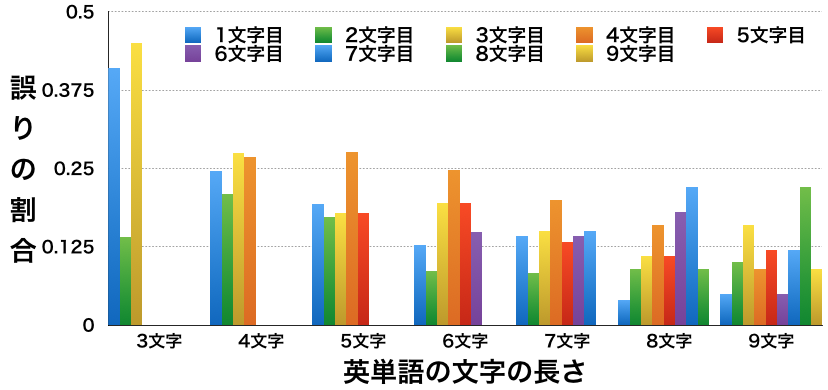
\includegraphics[width=8cm]{graph.png}
		\caption{単語内のスペリング誤りの位置の割合}
		\label{LabelExa}
\end{figure}

 \begin{table}[t]
  \small
   \centering
   \caption{単語同士を見間違えた例と同じスペリング誤りを繰り返した場合の例}
   \begin{tabular}{|c|c|} \hline
       	ユーザが入力した文字列 & 文字列に対応した英単語\\ \hline
	    th\underline{r}ough & though\\ \hline
	    he\underline{a}r\underline{h}e & here\\ \hline
	    sti\underline{gg}ff & stiff\\ \hline
	    s\underline{e}w\underline{wt}eet & sweet\\ \hline
   \end{tabular}
 \end{table}

\subsubsection{同じスペリング誤りが連続している場合}
タイピングゲームにおいて同じ文字が連続しているような英単語が表示されたとき,その文字列に対して同じスペリング誤りを繰り返してしまうといった事例が見られた.表5では英単語stiffに対してユーザが文字列sti\underline{gg}ffを入力した場合を示しており,これは文字fに対して文字gを入力してしまっている.このスペリング誤りはキーボードの配置による打鍵誤りによるものだと考えられ,同じ文字が連続している文字列に対してスペリングを誤った場合,同様のスペリング誤りを繰り返してしまう傾向にあると考えられる.

また文字と文字列のアルファベットが入れ替わる場合がある.表5では英単語sweetに対してユーザが文字列s\underline{e}w\underline{wt}eetを入力していて,この場合ユーザは文字wを入れようとしているときに文字eを,文字列eeを入れようとしているときに文字列wwを入力してしまっていると考えられる.この事例から文字と文字同士だけでなく,文字列と文字列同士のアルファベットの入れ替わりが起こりうることを示している.

\section{おわりに}
本研究ではユーザがタイピングゲームを行うことでスペリング誤りを抽出する手法を提案した.ユーザ7名にタイピングゲームのプレイを依頼し,4,724回の英単語タイピングログを収集し,859個のスペリング誤りを抽出した.抽出されたスペリング誤りに対して分析を行うことで,タイピングゲームのような通常より素早くタイピングを行ったり,文字を書き写すような状況では,キー配置によって起こる誤りや入力すべき文字を飛ばしてしまう誤りがよく起きることがわかった.

しかし本研究での実験設定ではユーザが入力しようとしている英単語はわかっているが,文字の挿入誤りと置換誤りの区別ができない.
区別を可能にするためには,Babaらの研究\cite{babaACL2012}のようにバックスペースを入力させて文字を消去させる必要があると考えられる.
また本研究での実験設定ではわからないが,ユーザによってスペリング誤りの頻度や傾向が変わっていることが考えられる.そのためタイピングゲームを行うときにユーザにアカウントを登録させてユーザそれぞれを区別できるようにすることで,ユーザごとの誤り訂正モデルの構築が可能であると考えられる.

今後はユーザに対して教育的であるようなデータセットの利用,実験設定を検討したい.
たとえば英語のリスニングゲームとしてタイピングゲームを発展させることで,新たなスペリング誤りの傾向の発見や研究において有用なログの作成,ユーザにとって有益となるようなコンテンツの構築に繋げていきたい.

\begin{comment}
\section*{謝辞}
実験を行うにあたりタイピングゲームをプレイして頂いたユーザ7名に対して深く感謝いたします.
\end{comment}

\bibliography{ai_gakkai}
\bibliographystyle{jsai}
%
\end{document}
